\documentclass[main.tex]{subfiles}

\begin{document}    
\addtocontents{toc}{\let\protect\contentsline\protect\nopagecontentsline}
\chapter{Fundamentals}\label{cpt:fun}
\addtocontents{toc}{\let\protect\contentsline\protect\oldcontentsline}

This chapter will cover the different topics required for understanding the analytical and numerical aspects of our parton shower formalism. Most of the results given in this chapter will be quoted from known texts, and formal derivations will generally not be recreated. The topics to be covered are quantum chromodynamics, jets, and kinematics of parton branchings. The first of these is a purely theoretical framework for the strong nuclear force, while the second will explore the concepts of jets. Kinematics of parton branchings will be focusing on the mathematics of simple parton branching in vacuum, and will be important when implementing them into Monte-Carlo programs. 

Natural units are used throughout the thesis such that \(\hbar = c = 1\).

\section{Quantum Chromodynamics}\label{sec: QCD}
Quantum chromodynamics (QCD) is the theory describing the strong interaction, one of the four fundamental forces in nature. It is a quantum field theory and a part of the famous standard model.

Historically there were several problems QCD tried to address. Among them was the ratio of the hadronic cross section to the muon-pair cross section produced by \(e^+e^-\)  interactions 
\begin{equation}
    R = \frac{\sigma(e^+e^-\rightarrow\text{hadrons})}{\sigma(e^+e^- \rightarrow \mu^+\mu^-)}
\end{equation}
which was off by a factor three in the calculation. Another issue yet to be addressed was the existence of the \(\Omega^-\) particle, consisting of three strange quarks, giving it a symmetrical wavefunction which violates the Pauli principle. It was also unclear at the time why members of the triplet representations of the SU(3) group, with fractional charges (\(\frac{2}{3}\) and \(-\frac{1}{3}\)), were unobserved in experiments~\cite{CERN_courier_History_of_QCD}. 

The addition of the color degree of freedom resolved all of these challenges. By allowing three different colors, the \(R\) ratio gained a factor of three. The \(\Omega^-\) could now have an anti-symmetric wavefunction as there was now another quantum number with three different values. The elusive fractionally charged hadrons were also accounted for by assuming that hadrons can only form as colorless states. This will be further explored in the section on confinement. As the name implies, quantum chromodynamics is the theory of color charges, and we will see that it is aptly named.

This section begins by exploring the basics of QCD. Covering how casimirs (color factors) originate from the generators of the SU(3) group, and giving a short overview of the Lagrangian and the first-order Feynman diagrams. Following that, a discussion on confinement will be given. Finally the concept of the running coupling, or asymptotic freedom, which defines how the strength of the strong interactions changes with scale and distance, will be introduced.

\subsection{The basics of QCD}
\subsubsection*{Group theory}
Formally quantum chromodynamics is a non-abelian gauge theory described by the SU(3) symmetry, which is a Lie group. The generators of the group are defined from the traceless hermitian Gell-Mann matrices \(\lambda_a\) defined as
\begin{align}\label{eqn: gell_mann_matrices}
    \begin{split}
    \lambda_1 = \mqty(0&1&0\\1&0&0\\0&0&0) \quad, \quad \lambda_2 &= \mqty(0&-i&0\\i&0&0\\0&0&0) \quad, \quad \lambda_3 = \mqty(1&0&0\\0&-1&0\\0&0&0), \\
    \lambda_4 = \mqty(0&0&1\\0&0&0\\1&0&0) \quad, \quad \lambda_5 &= \mqty(0&0&-i\\0&0&0\\i&0&0) \quad ,\\
    \lambda_6 = \mqty(0&0&0\\0&0&1\\0&1&0) \quad ,\quad \lambda_7 &= \mqty(0&0&0\\0&0&-i\\0&i&0) \quad, \quad \lambda_8 = \mqty(1&0&0\\0&1&0\\0&0&-2)\frac{1}{\sqrt{3}}.
    \end{split}
\end{align}
The generators \(T^a\) of QCD satisfy the Lie Algebra of the SU(3) group \(\left[T^a, T^b\right] = i \, f^{abc}\, T^c\). Where \(f^{abc}\) is the \emph{structure constants}. Physicists generally normalize the structure constants as \(\sum_{c,d}f^{acd}\, f^{bcd} = N \delta^{ab}\), where \(N\) is the number of colors. The normalization of the generators follows naturally as~\cite[p.485]{schwartz2014quantum},
\begin{equation}\label{eqn: color_operators}
    T^a = \frac{1}{2}\, \lambda_a \quad, \qquad (a=1,2,\cdots, 8).
\end{equation}
The generators are also called \emph{color operators} as they act on the color wavefunctions \(\chi^c\). For a single quark the wavefunction is written as a product of the space/spin wavefunction \(\psi\), and the color wavefunction \(\chi^c\) represented by the color spinors, 
\begin{equation}\label{eqn: color_spinors}
    r = \mqty(1\\0\\0) \quad, \quad g = \mqty(0\\1\\0) \quad, \quad b = \mqty(0\\0\\1).
\end{equation}
When examining the color operators it can be noted that only two of them commute, \(T^3\) and \(T^8\). The color states \(\chi^c =a,b,c\) are therefore eigenstates of both these operators and do not change if acted on by \(T^3\) or \(T^8\). The remainder of the color operators are non-diagonal and can therefore change color states, which means that the interaction can annihilate quarks of one color, and create quarks of a different color. It is therefore implied, by conservation of color, that gluons must have non-zero color charges, and therefore be able to self-interact. 

The color operators will inevitably allow us to introduce eight real gauge fields \(\mathbf{A}^\mu = A^{\mu a}\, \lambda^a\), where \(a=(1,2,\cdots,8)\), which corresponds to the octet of vector gauge bosons - the eight gluon fields.

The generators as presented here define the fundamental representation of the SU(3) group, meaning that it is the smallest non-trivial representation of the algebra. It is the most important representation, along with the adjoint representation described by \((T^a_{\text{adj}})^{bc}=-if^{abc}\). Different representations can be characterized in a basis-independent way using \emph{casimirs}. The quadratic casimir of a representation \(R\) is defined, \(T_R^aT_R^a = C_2(R) \mathbf{1}\). For evaluating the quadratic casimir, it will be useful to define an inner product for the generators as \(\text{tr}\left[T_R^aT_R^b\right]=T(R)\delta^{ab}\). The number \(T(R)\) is then known as the index of the representation. For a given SU(N) group the index \(T_R\equiv T(R)\) and quadratic casimir \(C_R\equiv C_2(R)\) of a given representation \(R\) is then given by~\cite[p.484-489]{schwartz2014quantum}. 
\begin{align}\label{eqn: casimirs}
    T_A = C_A = N \quad, \qquad T_F = \frac{1}{2}  \quad, \qquad C_F = \frac{N^2-1}{2N}.
\end{align}
These quantities appear in almost every QCD calculation.

\subsubsection*{The QCD Lagrangian}
Since QCD is a quantum field theory it has a \emph{Lagrangian} which describes the free and interacting parts of the particle fields. We will not do any formal derivation, but will be motivating the relevant results given by standard textbooks. QCD is described by the Yang-Mills Lagrangian~\cite{Peskin:1995ev},
\begin{align}\label{eqn: yangmills_lagrangian_mandlshaw_11.35}
    \mathcal{L}_{\textit{QCD}} &= \bar \Psi^f(x) \left[ i \slashed D -m_f \delta_{ij}\right] \Psi^f(x) - \frac{1}{4} G_{i\mu\nu}(x)G_{i}^{\mu\nu}(x)
\end{align}
where \(f = (1,\cdots, N_f)\) is a flavor index. The gluon term and covariant derivative is defined as 
\begin{align}
    G_i^{\mu\nu}(x) &= \partial^\nu A_i^\mu(x) - \partial^\mu A_i^\nu(x) + g_s f_{ijk}A_j^\mu(x)A_k^\nu(x) \\
    D^\mu \Psi^f(x) &= \left[\partial^\mu + ig_s \lambda_j A_j^\mu(x)/2 \right]\Psi^f(x)
\end{align}
where \(i,j = (1,2,\cdots,8)\). The gluon term corresponds to free gluons, with an additional interaction term for achieving gauge-invariance. The covariant derivative then ensures invariance under local phase transformations. The Lagrangian of \autoref{eqn: yangmills_lagrangian_mandlshaw_11.35} is therefore gauge invariant, and not suitable for quantization as the path integral formulation gives no methods for selecting among equivalent solutions. This is resolved by the Faadeev-Popov method which fixes the choice of gauge by adding a gauge fixing term to the Lagrangian~\cite{mandl2010quantum}. We will now explore two of the most common gauges, the \emph{Feynman gauge}, and the \emph{light-cone gauge}.

\subsubsection*{Feynman gauge}
The first type of gauges we will examine are the covariant \(R_\xi\) gauges introduced by the gauge fixing
\begin{equation}\label{eqn: gauge_fixing_Rxi}
    \mathcal{L}_{\text{gauge-fix}} = -\frac{1}{2\lambda} \left(\partial_\mu A_i^\mu(x)\right)^2.
\end{equation}
These gauges preserve Lorentz invariance and give simpler calculations than non-covariant gauges. We will be working with the Feynman gauge, commonly used in field theory calculations, which is obtained by setting \(\lambda =1\) in the gauge fixing.

The consequence of choosing covariant gauges is that we are no longer guaranteed that only physical transverse modes of \(A_\mu^a\) propagate, and we obtain additional kinetic terms which are ghost-like, giving us ghost fields \(\eta_i(x)\). These fields correspond to unphysical spin-0 fermions which can only appear as virtual particles in loop corrections ~\cite{schwartz2014quantum, mandl2010quantum}. Introducing the gauge-fixing term of the Feynman gauge and resulting ghost fields gives the following Lagrangian
\begin{align}\label{eqn: QCD_Lagrangian_feynman_gaugefixghost}
    \begin{split}
    \mathcal{L}_{\textit{QCD}} &= \bar \Psi^f(x) \left[ i \slashed D -m_f\right] \Psi^f(x) - \frac{1}{4} G_{i\mu\nu}(x)G_{i}^{\mu\nu}(x) \\
    &\quad - \frac{1}{2\lambda} \left( \partial_\mu A_i^\mu(x)\right)^2 + \partial_\nu \eta_i(x) \left[\partial^\nu \tilde \eta_i(x)+g_s f_{ijk} \tilde\eta_j(x) A_k^\mu(x)\right].
    \end{split}
\end{align}
The gluon propagator in the Feynman gauge is given as
\begin{equation}\label{eqn: gluon_propagator_feynman}
    i \Pi_{\text{feynman}}^{\mu\nu ab} = \frac{-i g^{\mu\nu}}{p^2+i\epsilon} \delta^{ab}.
\end{equation}

\subsubsection*{The light-cone gauge}
Turning to the light-cone gauge which is a type of axial gauge. Axial gauges violate Lorentz invariance, and makes it such that ghosts decouple from the physical particles, and can be ignored altogether. The gauge fixing of axial gauges is given by
\begin{equation}\label{eqn: gauge_fixing_axial}
    \mathcal{L}_{\text{gauge-fix}} = -\frac{1}{2\lambda} \left(n_\mu A_i^\mu(x)\right)^2,
\end{equation}
where \(n_\mu\) is some vector. The light-cone gauge is then defined from \(n^2 = 0\) and \(\lambda = 0\), meaning that \(n_\mu\) is light-like. The gluon propagator in the light-cone gauge is given as
\begin{equation}\label{eqn: gluon_propagator_lightcone}
    i \Pi_{\text{light-cone}}^{\mu\nu ab} = \frac{i}{p^2+i\epsilon} \left[-g^{\mu\nu}+ \frac{n^\mu p^\nu+p^\mu n^\nu}{np} \right]\delta^{ab}.
\end{equation}
There are only two physical polarizations in the light-cone gauge, those transverse to the \(n-p\) plane. The numerator of the propagator is the polarization sum of transverse modes in a given basis, since there are only two propagating polarizations, we don't need ghosts to eliminate unphysical polarizations.  

Axial gauges are not really useful unless there is some natural direction to choose. It is therefore very applicable in heavy-ion collisions, as we generally have an initial parton travelling in some direction which can define the vector \(n_\mu\). 

\subsubsection*{Feynman diagrams}
Since we are generally concerned with interactions it is possible to expand the terms of our Lagrangian in the Feynman gauge, \autoref{eqn: QCD_Lagrangian_feynman_gaugefixghost}, and isolate the interaction parts of the Lagrangian for quarks, gluons, and ghosts, respectively as:
\begin{align}
    \mathcal{L}_{\mathcal{I}\,\text{quark}} &= - \frac{1}{2} g_s \bar \Psi^f(x) \gamma_\mu \lambda_j \Psi^f(x) A_j^\mu (x) \label{eqn: QCD_Lpart_quark}  \\
    \begin{split}
    \mathcal{L}_{\mathcal{I}\,\text{gluon}} &= g_s f_{ijk} A_{i\mu}(x)A_{j\nu}(x) \partial^\mu A_k^\nu(x) \\
    &\quad - \frac{1}{4} g_s^2 f_{ijk} f_{ilm} A_j^\mu(x) A_k^\nu(x) A_{l\mu}(x) A_{m\nu}(x) \label{eqn: QCD_Lpart_gluon} \end{split} \\
    \mathcal{L}_{\mathcal{I}\,\text{ghost}} &= g_s f_{ijk} (\partial_\mu \eta_i(x)) \Tilde{\eta}_j(x) A_k^\mu(x). \label{eqn: QCD_Lpart_ghost} 
\end{align}
From these interaction-terms the famous Feynman diagrams can be obtained. \autoref{eqn: QCD_Lpart_quark} gives us a single three-point vertex which gives rise to two diagrams (depending on how the contraction is done), with two quarks and one gluon in each. The diagrams are pictured in \autoref{fig: feynman_quark_interactions}. The gluon contribution to the lagrangian gives us two different terms containing exclusively gluon fields, demonstrating the gluon self-interaction we expected from the color operators. The result is the three-gluon vertex and the four-gluon vertex as pictured in \autoref{fig: feynman_gluon_interactions}. The ghost term also gives rise to a Feynman diagram, which we have not printed here, as it can only occur in virtual loops and can be completely neglected in the light-cone gauge.
\begin{figure}[htb]
    \centering
    \begin{minipage}{.35\textwidth}
    \centering
        \begin{tikzpicture}
            \begin{feynman}
            \vertex (a);
            \vertex [right=of a] (v);
            \vertex [above right=of v] (b);
            \vertex [below right=of v] (c);
            \diagram* {
            (a) -- [gluon, edge label = \(k_1 \) ] (v),
            (v) -- [fermion, edge label' = \(k_2 \) ] (b),
            (v) -- [anti fermion, edge label = \(k_3 \) ] (c),
            };
            \end{feynman}
        \end{tikzpicture}
  \label{fig:test1}
\end{minipage}%
\begin{minipage}{.35\textwidth}
    \centering
        \begin{tikzpicture}
            \begin{feynman}
            \vertex (a);
            \vertex [right=of a] (v);
            \vertex [above right=of v] (b);
            \vertex [below right=of v] (c);
            \diagram* {
            (a) -- [fermion, edge label = \(k_1 \) ] (v),
            (v) -- [fermion, edge label' = \(k_2 \) ] (b),
            (v) -- [gluon, edge label = \(k_3 \) ] (c),
            };
            \end{feynman}
        \end{tikzpicture}
\end{minipage}
\caption{Tree-level Feynman diagrams for the quark contributions in the QCD Lagrangian.}
\label{fig: feynman_quark_interactions}
\end{figure}
\begin{figure}[htb]
    \centering
    \begin{minipage}{.35\textwidth}
    \centering
      \begin{tikzpicture}
            \begin{feynman}
            \vertex (a);
            \vertex [below=of a] (v);
            \vertex [below right=of v] (b);
            \vertex [below left=of v] (c);
            \diagram* {
            (a) -- [gluon, edge label = \(k_1 \) ] (v),
            (b) -- [gluon, edge label' = \(k_2 \) ] (v),
            (c) -- [gluon, edge label = \(k_3 \) ] (v),
            };
            \end{feynman}
        \end{tikzpicture}
\end{minipage}%
\begin{minipage}{.35\textwidth}
    \centering
        \begin{tikzpicture}
            \begin{feynman}
            \vertex (a);
            \vertex [below right=of a] (v);
            \vertex [above right=of v] (b);
            \vertex [below right=of v] (c);
            \vertex [below left=of v] (d);
            \diagram* {
            (a) -- [gluon, edge label' = \(k_1 \) ] (v),
            (b) -- [gluon, edge label = \(k_4 \) ] (v),
            (c) -- [gluon, edge label' = \(k_3 \) ] (v),
            (d) -- [gluon, edge label = \(k_2 \) ] (v),
            };
            \end{feynman}
        \end{tikzpicture}
\end{minipage}
\caption{Tree-level Feynman diagrams for the gluon contributions in the QCD Lagrangian. Three-gluon vertex (left), and four gluon vertex (right).}
\label{fig: feynman_gluon_interactions}
\end{figure}

These are all of the \(\mathcal{O}(g)\) interactions of QCD. There are naturally higher-order diagrams and loop-corrections which may pose challenges when dealing with calculations, but for our purposes the first-order terms are sufficient. This allows us to disregard the four-gluon vertex in later sections as it is \(\sim g^2\). 

\subsection{Confinement}
Confinement is the phenomenon that particles with color charge does not exist as isolated particles under normal conditions of temperature and pressure. While it is not clear how it emerges from the Lagrangian of QCD, it remains an experimental fact - quarks and gluons are forced to be bound into color-neutral states called hadrons~\cite{Caucal:2020zcz}. The simplest example is mesons which consist of a quark and an anti-quark of the same flavor which is a color-neutral state. 

The familiar Coulomb potential of QED is attractive for opposite charges, and repulsive for similar charges. It would therefore be interesting to observe how the QCD potential behaves for \(q \bar q\)-pairs, of similar and different color charge. For large separations the potential increases linearly \(V(r) \sim k\, r\), while at small separations a potential similar to the Coulomb will dominate. This calculated in~\cite[p.512-513]{schwartz2014quantum}, and the QCD potential can then be written as
\begin{align}\label{eqn: QCD_potential}
    \begin{split}
    V_{\text{QCD}}(r) &= k\,r - \frac{4}{3} \frac{g_s^2}{4\pi r} \quad, \qquad \text{(color singlet)}, \\
    V_{\text{QCD}}(r) &= k\,r + \frac{1}{6} \frac{g_s^2}{4\pi r} \quad, \qquad \text{(color octet)}.
    \end{split}
\end{align}
The color singlet represents the potential for \(q \bar q\)-pairs of the same color charge and is the only one attractive at small separations. This is consistent with our expectations that quarks can form color-neutral mesons. The color octet, which gives all combinations of \(q \bar q\)-pairs of different color charge, is however repulsive for all \(r\), and mesons with a net color charge does not form. 

An interesting part of confinement should become apparent when examining the potential between a \(q \bar q\)-pair of similar color charge. If we were to forcefully separate the quarks, the potential between them would eventually become large enough for it to be energetically favorable to form a new \(q \bar q\)-pair which then combine with the existing pair, giving us two mesons. This property is illustrated by the famous rubber band analogy in \autoref{fig: QCD_rubberband}. 
\begin{figure}[htb]
    \centering
    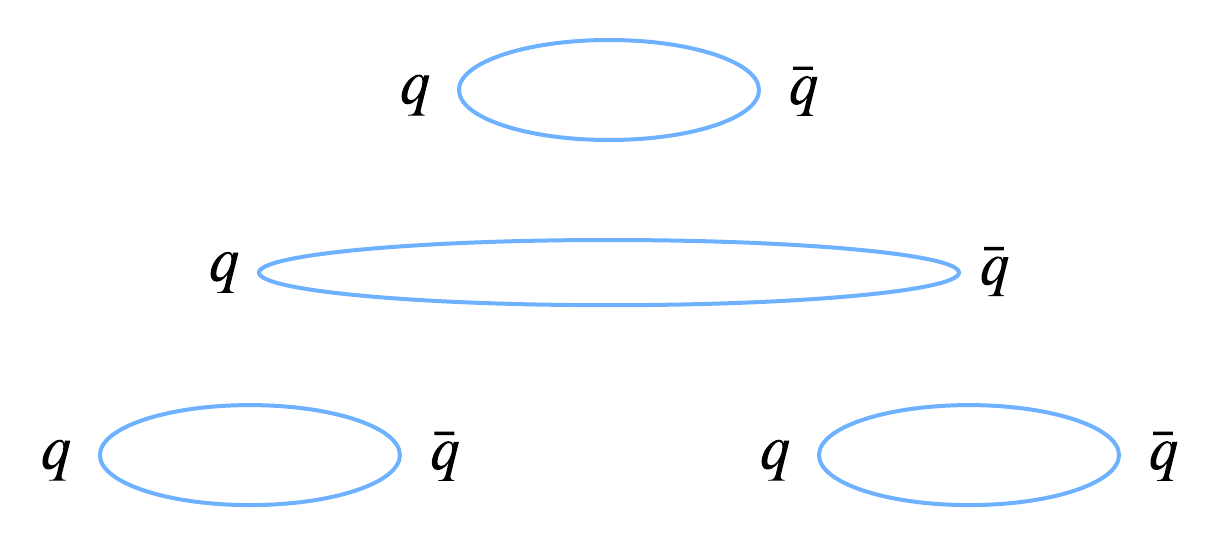
\includegraphics[width=9cm]{pictures/figures/QCD_potential_rubberband.png}
    \caption{When the potential between a \(q\bar q\)-pair becomes too large, it is energetically favorable to create a new \(q\bar q\)-pair. This can be visualized as pulling a rubber band that instead of breaking, spontaneously turns into two new rubber bands.}
    \label{fig: QCD_rubberband}
\end{figure}

\subsection{The running coupling}
Field theories such as QED and QCD, have a coupling constant describing the strength of a given interaction, relative to the free fields. For QED this is the fine-structure constant \(\alpha \approx \frac{1}{137}\), which is proportional to the squared electric charge \(e^2\), which we can intuitively associate with how strongly an electrically charged particle interacts with an electric field. The same goes for QCD, where the coupling constant \(g_s\) only appears in the interaction-parts of the Lagrangian. higher-order interactions scale with orders of the coupling constant, as is apparent in \autoref{eqn: QCD_Lpart_gluon} where the three-gluon vertex is scaled by \(g_s\), and the four-gluon vertex is scaled by \(g_s^2\). 

The QCD Lagrangian given by \autoref{eqn: yangmills_lagrangian_mandlshaw_11.35} contains the bare coupling constant \(g_s\). This is only valid for tree-level in perturbation theory, and needs to be corrected by the method of \emph{renormalization} to account for divergences appearing from higher-order loop corrections. Renormalization will allow us to replace the bare coupling constant with a renormalized coupling constant \(g_r(\mu)\), where \(\mu\) is an scale dependence appearing as a consequence of the renormalization procedure. It is customary to define this new coupling in analogy to the fine-structure constant such that \(\alpha_s(\mu)=\frac{g_r^2}{4\pi}\), the new coupling can be written to leading order as
\begin{equation}\label{eqn: coupling_QCD_running}
    \alpha_s(\mu) = \frac{2\pi}{\beta_0 \ln(\mu^2/\Lambda_{\text{QCD}}^2)}.
\end{equation}
In this coupling \(\beta_0\) is the leading order expansion of the full \emph{\(\beta\)-function}, which encodes how the coupling changes with scale. The \(\beta\)-function is therefore responsible for the running of the coupling constant. \(\Lambda_{\text{QCD}}\) is the scale at which the coupling constant becomes infinite, also called the Landau pole, and for QCD this scale is typically \(\Lambda_{\text{QCD}} \sim 0.2 \text{ GeV}\).

The importance of the running coupling in QCD is that \(\alpha_s(\mu)\rightarrow 0\) as \(\mu\rightarrow \infty\). This is known as \textit{asymptotic freedom}. For processes with a large momentum transfer \(Q>>\Lambda_{\text{QCD}}\), such as high energy jets, the process can be described by perturbation theory. The uniqueness of the running coupling in QCD is that the \(\beta\)-function is negative, which gives rise to confinement~\cite{Caucal:2020zcz}.

\subsection{Quark-gluon plasma}
In our discussion on confinement we made an explicit statement that particles with color charge can not exist as isolated particles under "normal conditions of temperature and pressure". This naturally sparks the question of what happens under extreme conditions with high temperature and high pressure.

At increasing temperature and/or increasing baryonic chemical potential, a phase transition occurs such that hadrons no longer exist. The resulting matter consisting of free quarks and gluons is commonly called a \emph{quark-gluon plasma} (QGP). While it is commonly called a plasma it is not always clear whether it should be interpreted as a weakly interacting gas or a strongly correlated system such as a fluid. 
The properties of the quark-gluon plasma is best illustrated using a phase diagram such as the one given in \autoref{fig: QCD_phasediagram}.
\begin{figure}[htb]
    \centering
    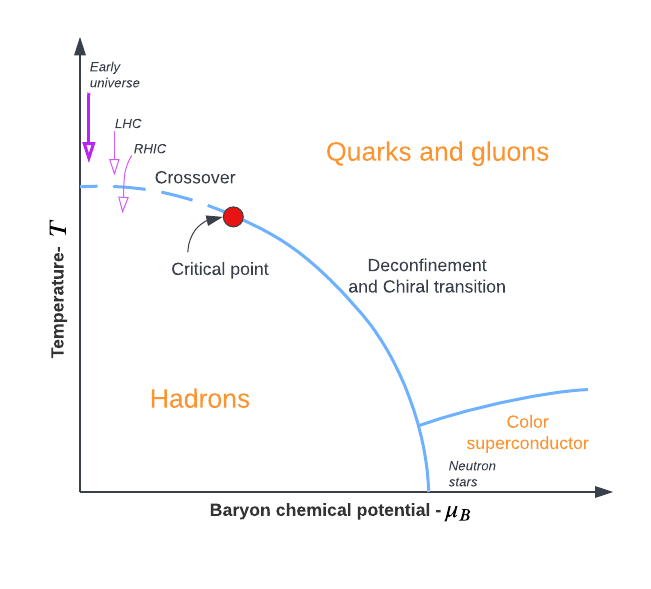
\includegraphics[width=10cm]{pictures/figures/QCD_phasediagram.png}
    \caption{Diagram for the phase transition from hadronic matter to quark-gluon plasma. The transition from hadrons to QGP is split into a crossover section, and a phase transition (deconfinement).}
    \label{fig: QCD_phasediagram}
\end{figure}

There are several points of interest in this phase diagram. The most obvious feature is the phase transition between the hadron gas and the quark-gluon plasma, at finite \(\mu_B\), which is an important feature of QGP. However, at the same point, there is also a \emph{chiral phase transition} happening. In short, chiral symmetry is broken in QCD, meaning that the theory acts differently on left and right-handed fields. This symmetry is restored for high pressure and/or temperature, and seemingly coincides with deconfinement when plotting the phase transitions in terms of the baryonic chemical potential. Another important feature is the \emph{crossover}, at high temperature and low baryonic chemical potential, where there is no well defined phase transition and the hadrons transform smoothly into a QGP, this is the region LHC operates at~\cite{florkowski2010phenomenology}. In the color superconducting phase the quarks are bound in Cooper pairs and form the SU(3) analogue of superconductivity~\cite{Fischer_2019}.

Studying the QGP is difficult as it is incredibly short-lived and difficult to measure directly. The main method of probing the quark-gluon plasma is to observe how highly energetic partons interact with the plasma in the immediate aftermath of heavy-ion collisions (\(Au+Au\)), at colliders such as RHIC and LHC. These high-energy particles lead to \emph{jets}.

\section{Jets}
A jet is a narrow cone of particles, produced by successive branchings of some initial parton created in the aftermath of particle collisions with extremely large momentum transfer, at colliders such as RHIC and LHC. The quarks and gluons created by parton branchings eventually hadronize and are observed in the detector as parton showers. The jets may propagate with or without a background medium. The former requires relativistic heavy-ion collisions, typically \(Pb\) or \(Au\), while the latter may be created by \(e^+e^-\)-collisions.

This section will discuss the properties of jets in both vacuum and medium, and the terminology associated with them. After that, we will introduce the observables relevant for this thesis.

\subsection{Jets in vacuum}
Starting with jets in vacuum. Since there is no background medium for the partons to interact with the picture is relatively simple, and we need only concern ourselves with basic parton branching.

\subsubsection*{Basic parton branching}
Parton branching is simply the process of an energetic parton splitting into two new partons. This can happen via all of the basic QCD vertices (\autoref{fig: feynman_quark_interactions} and \autoref{fig: feynman_gluon_interactions}) and allows for the number of partons in a jet to increase, which eventually leads to the parton showers we observe in the detector. When addressing parton branching we will generally mean \emph{soft} and \emph{collinear} branching. In soft branching the emitted parton carry very little transverse momentum \(z\), relative to the parent parton. Collinear branching is when the newly created parton travels in roughly the same direction as the branching parton, implying that the opening angle \(\theta\) of the branching is very small. Soft and collinear branching will appear as divergences in the branching probability proportional to
\begin{align}
    \mathcal{P}_{\text{branching}} \sim \frac{\alpha_s}{\pi} \frac{d\theta}{\theta} \frac{dz}{z}.
\end{align}
This will be derived in \autoref{sec: kinematics}.

\subsubsection*{Angular ordering}
The parton showers evolving without a background medium will be angular ordered, meaning that any subsequent emission angle is smaller than the previous angle. For simple parton branchings, angular ordering can be obtained by considering the spatial separation of the daughter-partons of the branching.
\begin{figure}[htb]
    \centering
        \begin{tikzpicture}
            \begin{feynman}
            \vertex (a);
            \vertex [right=1.0cm and 3.3cm of a] (a1);
            \vertex [above right=0.85cm and 1.5cm of a1] (b1);
            \vertex [below right=0.85cm and 1.5cm of a1] (b2);
            \vertex [above right=0.85cm and 1.5cm of b1] (c1);
            \vertex [below right=0.85cm and 1.5cm of b2] (c2);
            \vertex [above right=0.85cm and 1.5cm of c1] (d1);
            \vertex [below right=0.15cm and 1.5cm of c1] (d2);
            \vertex [above right=0.85cm and 1.5cm of d1] (e1);
            \vertex [below right=0.15cm and 1.5cm of d2] (e2);
            \vertex [below = 0.22cm of c1] (r1);
            \vertex [above = 0.22cm of c2] (r2);
            \diagram* {
            (a) -- [gluon, edge label = \(a\)] (a1),
            (a1) -- [gluon, edge label = \(c\)] (e1),
            (c2) -- [gluon, edge label = \(b\)] (a1),
            (e2) -- [gluon, edge label = \(d\)] (c1),
            (d2) -- [scalar, quarter right,opacity = 0.6, edge label = \(\theta \) ] (d1),
            (b2) -- [scalar, quarter right,opacity = 0.6, edge label = \(\theta_0 \) ] (b1),
            (r1) -- [ghost, opacity = 0.5, edge label = \(r_\perp\)] (r2),
            };
            \end{feynman}
        \end{tikzpicture}
\caption{Illustration of the opening angles for successive parton branchings. The branching is said to be resolvable if the separation distance \(r_\perp\) at the time \(t_f\) of the second branching is larger than the wavelength of the emitted gluon \(d\).}
\label{fig: angular_ordering}
\end{figure}

Looking at \autoref{fig: angular_ordering}, we have noted the opening angle as \(\theta_0\) for the initial branching, and \(\theta\) for the successive branching. If the secondary branching parton has a wavelength \(\lambda \sim \frac{1}{k_\perp} \sim \frac{1}{\omega \theta}\), with formation time \(t_f\sim \omega/k_\perp^2\), then the formation time can be written
\begin{equation}
    t_f \sim \frac{\omega}{k_\perp^2} = \frac{1}{\omega \theta^2}.
\end{equation}
The spatial separation of the partons from the initial branching can be given from the same formation time as \(r_\perp \sim \theta_0\, t_f = \frac{\theta_0}{\omega \theta^2}\). Demanding that the wavelength \(\lambda\) of the branched parton \(d\) must be smaller than the separation distance \(r_\perp\) we obtain
\begin{align}\label{eqn: angular_ordering}
    \lambda &< r_\perp \nonumber \\
    \frac{1}{\omega \theta} &< \frac{\theta_0}{\omega \theta^2} \nonumber \\
    \theta &< \theta_0.
\end{align}
The criteria \(\lambda < r_\perp\) leads us therefore to angular ordering. The reason we are able to impose this criterion originates from our desire to have \emph{resolvable} branchings. This means that the branched parton \(d\) should be able to probe whether it branched from \(c\), or from \(b\). This is also called \emph{coherent branching}. If the wavelength of \(d\) is too large, then it will not be able to distinguish \(b\) and \(c\) as individual partons, and it would instead branch from the sum of the color charges, which is equivalent to branching from \(a\)~\cite{Dokshitzer:1991wu}. When we are constructing our Monte-Carlo program we will be using the angle \(\theta\) as our ordering variable, meaning that we start from a large value of \(\theta\) and branch our way down to smaller angles. Angular ordering follows therefore naturally from the choice of evolution variable.

Coherent branching also imply that color charge is conserved along the parton shower for the same reasons - if the branching is resolvable each successive branching will conserve the net color charge. 

\subsection{Jets in medium}
Jets traversing a background medium, typically QGP formed in the aftermath of heavy-ion collisions, bring along some more complex phenomena. Highly energetic partons interacting with the medium give rise to the phenomena of \emph{induced gluon radiation}, \emph{broadening}, and \emph{quenching}. All of these properties will be discussed, but first, we must take a closer look at how relativistic heavy-ion collisions evolve.

\subsubsection*{Evolution of relativistic heavy-ion collisions}
The different phases of relativistic heavy-ion collisions is given in \autoref{fig: evolution-heavy-ion-collisions}. The units of the diagram is \(fm/c\sim 10^{-24}s\). The first stage of the evolution is the pre-equilibrium dynamics where partons (mostly gluons) are quickly freed by the collision, and then start to approach thermal equilibrium. This gives us an initial energy density around \(1fm/c\) which is the basis for the quark-gluon plasma phase which evolves until around \(10fm/c\). When the pressure and temperature become too small for deconfinement, hadrons are formed in a process called \emph{hadronization}. The hadron gas is treated using relativistic hydrodynamics until it cools enough for the \textit{freeze-out}, which finally leaves us with the free hadrons we can observe in our detector. 
\begin{figure}[htb]
    \centering
    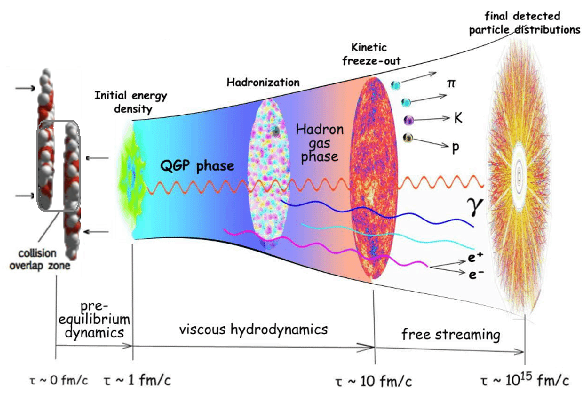
\includegraphics[width=12cm]{pictures/figures/evolution-of-relativistic-heavy-ion-collisions.png}
    \caption{Illustration of the evolution of relativistic heavy-ion collisions. Evolution starts at the initial collision and continues until the hadronized particles reach the detector. The bottom axis gives the time scale of the evolution, units \(fm/c \sim 10^{-24}s\), and the dynamics governing the system. This thesis concerns itself primarily with the QGP phase, evolving from the initial energy density to the hadronization. Figure from~\cite{QCD_figures/Scharenberg} but colors are inverted.}
    \label{fig: evolution-heavy-ion-collisions}
\end{figure}

When discussing jets in medium, we are interested in the high-energy partons at the very start of the QGP phase, and how they interact with the medium. These will lead to hadronization and eventually the parton showers we observe in the detector, which will be quite different from the jets evolving without a medium.

\subsubsection*{Gluon radiation}
Induced gluon radiation is very similar to the simple parton branchings discussed for vacuum cascades, but it is created by the jet interacting with the QGP and radiating soft gluons. These soft gluons are produced in abundance when jets move through a background medium. This happens via multiple collisions between the parton and the medium constituents, resulting in induced gluon radiation with a formation time of
\begin{equation}\label{eqn: induced_gluon_radiation_formationtime}
    t_f\sim \omega/k_\perp^2.
\end{equation}
These soft gluons carry very little momentum, and are typically emitted at large angles - the softer the emission, the larger the emission angle.
This leads to incoherent branchings, as the newly emitted partons will probe the net color charge. Color is therefore not necessarily conserved along the shower, and angular ordering is no longer the norm~\cite{medium_induced_gluon_branching}. 

\subsubsection*{Jet broadening}
Broadening takes place during the QGP phase of heavy-ion collisions. The concept is simply gluons exchanging transverse momentum with the medium, resulting in a broader transverse momentum distribution. 

During the time-scale of soft gluon emissions, the gluon can experience multiple kicks and gain transverse momentum on the scale of \(k_\perp^2 \sim \hat q \,t_f\). Here \(\hat q\) is a diffusion coefficient, called the \emph{jet-quenching parameter}, representing how the partons interact with the medium. \(\omega\) is the energy of the radiated gluon, and \(k_\perp\) is its transverse momentum relative to the parent gluon. If these kicks from the medium are the only source of transverse momentum then the formation time can be written in terms of the jet-quenching parameter
\begin{equation}\label{eqn: branching_time}
    t_f = \sqrt{\frac{\omega}{\hat q}}
\end{equation}
and can also be called the branching time. When the collisions are soft, and a large number of collisions is needed to change the transverse momentum by a significant amount, the diffusion approximation given by \(\hat q\) is valid. The total transverse momentum \(k_\perp\) gained by a high-energy parton traversing a medium of length \(L\) is therefore given From the definition of the diffusion coefficient as
\begin{equation}\label{eqn: broadening}
    \langle k_\perp^2\rangle = \hat{q}\, L.
\end{equation}
The jet-quenching parameter will generally be set to some constant, even though it is a function of momentum~\cite{Jet_Structure_HeavyIonCollisions}. Quenching is understood as the suppression of high \(p_T\) hadrons due to energy-loss from the most energetic parton of a given jet, commonly known as the leading parton. This energy-loss is primarily caused by soft gluon radiation, which is induced by collisions with the medium~\cite{medium_induced_gluon_branching}. The concepts of broadening and quenching are closely connected, and both are consequences of medium interactions.

\subsection{Observables}
This section will present different observables and quantities which will be particularly important for our treatment of parton showers. Before going into specific observables, it is necessary to define the transverse momentum \(p_t\) of the initial parton in a given jet, by the transverse momentum it has in the lab frame \(p_T\), such that \(p_t \equiv p_T\).

\subsubsection*{The jet radius}
The method of grouping different quarks and gluons into the same jet is defined by \textit{jet algorithms}. A recombination algorithm can be made by grouping any quarks or gluons separated by a distance 
\begin{align}
    \Delta_{ij}^2 = ((y_i-y_j)^2+(\phi_i-\phi_j)^2) < R^2
\end{align} 
into a single jet. Here \(y_i\) and \(\phi_i\) is the rapidity and azimuth of particle \(i\), and \(R\) is the \textit{jet radius}. The jet radius is not an observable for out showers, but it is an important quantity which must be defined for both numerical and analytical purposes~\cite{Dasgupta_2015}.

\subsubsection*{The inclusive parton distribution}
The observable we will encounter most frequently is the inclusive parton distribution. For a jet evolving according to an arbitrary evolution variable \(t\), the inclusive parton distribution is given as
\begin{align}
    f_i(x,t) = \frac{dN_i}{dx}
\end{align}
where \(i = (g,q,\bar q)\) labels the species of the parton, and \(x\) is its transverse momentum relative to the initial parton. The inclusive parton distribution then gives us any partons within a given energy range, at a given time of the evolution, evolving according to some evolution variable. The choice of evolution variable is somewhat arbitrary, common choices are momentum \(t = p_t^2\), scale \(t\sim \ln \frac{Q^2}{Q_0^2}\), and angle \(t\sim \ln \frac{\theta_{\text{max}}^2}{\theta_{\text{min}}^2}\). We will discuss the evolution variable at length in \autoref{cpt:ana}.
\begin{figure}[htb]
    \centering
    \begin{tikzpicture}
    \draw[dashed, opacity = 0.12] (0.05,-3) -- (0.05,3);
    \node[opacity =0.8] at (0.05,-3.3cm) {\(t_{0}\)};
    \draw[dashed, opacity = 0.12] (6.15,-3) -- (6.15,3);
    \node[opacity =0.8] at (6.15,-3.3cm) {\(t'\)};
    \draw[color = blue, dashed, opacity=0.5] (6.34cm,0) circle [x radius=0.38cm,y radius=0.7cm];
    \node[color = blue, opacity =0.8] at (7.45cm,0.5cm) {\(f_q(x_4,t')\)};
    \draw[color = black!30!green, dashed, opacity=0.8] (6.34cm,2.8) circle [x radius=0.38cm,y radius=0.7cm];
    \node[color = black!30!green, opacity =0.6] at (7.45cm,3.3cm) {\(f_g(x_1,t')\)};
    \begin{feynman}
            \vertex (a)  {};
            \vertex [right=2.5cm of a ] (a1);
            \vertex [above right=1.0cm and 1.2cm of a1] (b1);
            \vertex [below right=1.0cm and 1.2cm of a1] (b2);
            \vertex [above right=0.9cm and 1.2cm of b1] (c1);
            \vertex [below right=0.4cm and 1.0cm of b1] (c2);
            \vertex [above right=0.7cm and 1.2cm of b2] (c3);
            \vertex [below right=0.9cm and 1.2cm of b2] (c4);
            \vertex [above right=0.7cm and 1.2cm of c1] (d1){\(x_1\)};
            \vertex [below right=0.15cm and 1.2cm of c1] (d2){\(x_2\)};
            \vertex [above right=0.3cm and 1.4cm of c2] (d3){\(x_3\)};
            \vertex [below right=0.4cm and 1.4cm of c2] (d4){\(x4\)};
            \vertex [above right=0.4cm and 1.2cm of c3] (d5);
            \vertex [below right=0.4cm and 1.2cm of c3] (d6){\(x_5\)};
            \vertex [above right=0.15cm and 1.2cm of c4] (d7){\(x_6\)};
            \vertex [below right=0.7cm and 1.2cm of c4] (d8){\(x_7\)};
            \diagram* {
            (a) -- [fermion, edge label = {\(E=p_t\)}] (a1),
            (a1) -- [fermion] (b1),
            (a1) -- [gluon] (b2),
            (b1) -- [gluon] (c1),
            (b1) -- [fermion] (c2),
            (b2) -- [gluon] (d6),
            (b2) -- [gluon] (c4),
            (c1) -- [gluon] (d1),
            (c1) -- [gluon] (d2),
            (c2) -- [gluon] (d3),
            (c2) -- [fermion] (d4),
            (c4) -- [gluon] (d7),
            (c4) -- [gluon] (d8),
            };
        \end{feynman}
\end{tikzpicture}
\caption{Illustration of the inclusive parton distribution \(f_i(x,t)\) in a shower with both quarks and gluons, evolving according to an arbitrary evolution variable \(t\). Since the inclusive distribution can give any of the relevant partons in a given energy range at give point \(t'\), we have highlighted \(f_g(x_1,t')\) and \(f_q(x_4,t')\). }
\label{fig: inclusive_parton}
\end{figure}

The inclusive parton distribution \(f_i(x,t)\) is described by the DGLAP evolution equations which will be introduced in \autoref{cpt:ana}. Some of the properties of the inclusive distribution are
\begin{align}
    \int_0^1 dx\, f_i(x,t) &= \langle N_{i}\rangle  \label{eqn: inclusive_function_properties_1}\\
    \int_0^1 dx\, x\,  f_i(x,t) &= 1. \label{eqn: inclusive_function_properties_2}
\end{align}
\autoref{eqn: inclusive_function_properties_1} follows from the definition of the inclusive parton distribution, and tells us that the integral over all momentum values in the inclusive parton distribution yields the total number of partons. Since the inclusive distribution gives us the number of partons, it must conserve the total momentum as given by \autoref{eqn: inclusive_function_properties_2}~\cite{Neill_2021}.

When we develop our Monte-Carlo shower program the outcome is a list of all final partons which makes it easy to find the number of particles in a given momentum interval \(\frac{dN_i}{dx}\) and the energy density \(x \frac{dN_i}{dx}\). The inclusive parton distribution is therefore ideal for comparing analytical and numerical results in our parton showers.

\subsubsection*{The leading parton distribution}
The leading parton distribution \(\mathcal{J}_i(x,t)\) contrasts the inclusive distribution as it only concerns itself with the parton with the highest momentum relative to the initial parton, at a given time of the evolution.
\begin{figure}[htb]
    \centering
    \begin{tikzpicture}
    \draw[dashed, opacity = 0.12] (0.05,-3) -- (0.05,3);
    \node[opacity =0.8] at (0.05,-3.3cm) {\(t_{0}\)};
    \draw[dashed, opacity = 0.12] (6.15,-3) -- (6.15,3);
    \node[opacity =0.8] at (6.15,-3.3cm) {\(t'\)};
    \draw[color = black!30!green, dashed, opacity=0.6] (6.34cm,0) circle [x radius=0.38cm,y radius=0.7cm];
    \node[color = black!30!green, opacity =0.8] at (7.6cm,0cm) {\(\mathcal{J}_g(x,t')\)};
    \node[color = black!30!green, opacity =0.8] at (8.2cm,0.5cm) {\(x_4 = \) max\(\left\{ x_i\right\};\)};
    \begin{feynman}
            \vertex (a)  {};
            \vertex [right=2.5cm of a ] (a1);
            \vertex [above right=1.0cm and 1.2cm of a1] (b1);
            \vertex [below right=1.0cm and 1.2cm of a1] (b2);
            \vertex [above right=0.9cm and 1.2cm of b1] (c1);
            \vertex [below right=0.4cm and 1.0cm of b1] (c2);
            \vertex [above right=0.7cm and 1.2cm of b2] (c3);
            \vertex [below right=0.9cm and 1.2cm of b2] (c4);
            \vertex [above right=0.7cm and 1.2cm of c1] (d1){\(x_1\)};
            \vertex [below right=0.15cm and 1.2cm of c1] (d2){\(x_2\)};
            \vertex [above right=0.3cm and 1.4cm of c2] (d3){\(x_3\)};
            \vertex [below right=0.4cm and 1.4cm of c2] (d4){\(x4\)};
            \vertex [above right=0.4cm and 1.2cm of c3] (d5);
            \vertex [below right=0.4cm and 1.2cm of c3] (d6){\(x_5\)};
            \vertex [above right=0.15cm and 1.2cm of c4] (d7){\(x_6\)};
            \vertex [below right=0.7cm and 1.2cm of c4] (d8){\(x_7\)};
            \diagram* {
            (a) -- [gluon, edge label = {\(E=p_t\)}] (a1),
            (a1) -- [gluon] (b1),
            (a1) -- [gluon] (b2),
            (b1) -- [gluon] (c1),
            (b1) -- [gluon] (c2),
            (b2) -- [gluon] (d6),
            (b2) -- [gluon] (c4),
            (c1) -- [gluon] (d1),
            (c1) -- [gluon] (d2),
            (c2) -- [gluon] (d3),
            (c2) -- [gluon] (d4),
            (c4) -- [gluon] (d7),
            (c4) -- [gluon] (d8),
            };
        \end{feynman}
\end{tikzpicture}
\caption{Illustration of the leading parton distribution, for a parton shower consisting exclusively of gluons, evolving according to an arbitrary evolution variable \(t\). Here it is assumed that \(x_4 = \text{max}\{x_1,x_2,\cdots,x_7\}\) and the leading parton distribution \(\mathcal{J}_g(x,t')\) is highlighted accordingly. }
\label{fig: leading_parton}
\end{figure}

In contrast to the inclusive parton distribution, the leading parton distribution \(\mathcal{J}(x,t)\) represents a well-defined object which has lost energy due to emissions. The sum rules for the leading parton distribution are
\begin{align}
    \int_0^1 dx\, \mathcal{J}_i(x,t) &= 1 \label{eqn: leading_function_properties_1}\\
    \int_0^1 dx\, x\,  \mathcal{J}_i(x,t) &= \langle x\rangle.  \label{eqn: leading_function_properties_2}
\end{align}
The number of partons is constant in the leading distribution, as can be seen from \autoref{eqn: leading_function_properties_1}, and the energy is not conserved as can be seen from \autoref{eqn: leading_function_properties_2}. Since we have an expression for the average energy contained in the leading parton, the energy-loss can be calculated from \(\langle x_{i} \rangle_\text{loss} = 1 -\langle x_{i}\rangle \), this will be revisited in \autoref{cpt:leading}~\cite{Neill_2021}. 

\section{Kinematics of Parton Branching in Vacuum}\label{sec: kinematics}
Taking a step back from the concepts of QCD and jets, this section will discuss the actual kinematics of parton branchings in vacuum. Beginning by introducing the basic kinematic variables, before we explore the properties and origin of the Alterelli-Parisi splitting functions by considering the matrix-elements of the different QCD vertices. Finally we will take a look at the branching probability by considering the cross sections of a given process.

Rather than obtaining a precise result to some fixed order in perturbation theory, we will aim for an approximate result by considering the kinematics of parton branchings, which will be valid to all orders, allowing us to introduce a parton shower picture that can be easily implemented into Monte-Carlo programs.

\subsection{Kinematic variables}
Before doing any calculations the basic kinematic variables must be introduced. Restricting ourselves to the variables which will be used throughout the later sections. We start by considering the branching \(a\rightarrow b,c\) under the assumption that \(p_b^2, p_c^2 << p_a^2\). For now, we will be ordering our showers with respect to the initial parton energy \(t \equiv p_a^2\). An illustration of a single branching is given in \autoref{fig: parton_branching1}. 
\begin{figure}[htb]
    \centering
    \begin{tikzpicture}
    \node[opacity =0.5] at (4.2cm,0.33cm) {\(\theta_b\)};
    \node[opacity =0.5] at (4.2cm,-0.33cm) {\(\theta_c\)};
    \begin{feynman}
            \vertex (a) [blob] {};
            \vertex [right=1.0cm and 2.5cm of a ] (a1);
            \vertex [right=1.0cm and 0.25cm of a1 ] (a11);
            \vertex [right=1.0cm and 1.5cm of a1] (a2);
            \vertex [right=1.0cm and 0.7cm of a2] (a3);
            \vertex [above right=0.6cm and 1.0cm of a1] (b1);
            \vertex [below right=0.6cm and 1.0cm of a1] (c1);
            \vertex [above right=1.2cm and 2.2cm of a1] (b2);
            \vertex [below right=1.2cm and 2.2cm of a1] (c2);
            \diagram* {
            (a) -- [gluon, edge label = \(a\)] (a1),
            (a11) -- [ghost] (a3),
            (a1) -- [gluon, edge label = \(b\)] (b2),
            (c2) -- [gluon, edge label = \(c\)] (a1),
            (b1) -- [scalar, quarter left,opacity = 0.5 ] (a2),
            (a2) -- [scalar, quarter left,opacity = 0.5 ] (c1),
            };
        \end{feynman}
\end{tikzpicture}
\caption{Branching of an outgoing gluon \(a\) from some initial blob, into two gluons \(b,c\). The opening angle is given as \(\theta = \theta_b+\theta_c\). }
\label{fig: parton_branching1}
\end{figure}

The opening angle is given as \(\theta = \theta_b+\theta_c\), and the energy carried by the branched partons is given relative to the energy of the parent parton such that \(E_b=z\,E_a\) and \(E_c=(1-z)\,E_a\). The relationships between \(z\) and the different energies can therefore be written as
\begin{equation}\label{eqn: branched_energy_fractions_ellis_5.2}
    z = \frac{E_b}{E_a} = 1- \frac{E_c}{E_a}.
\end{equation}
Assuming most of our emissions are \emph{collinear}, the opening angle \(\theta\) is small, and we can use the small-angle approximations \(\cos \theta \approx 1- \frac{\theta^2}{2}\) and \(\sin \theta \approx \theta\). Conservation of four-momentum can be used to derive the following relationships between the kinetic variables - assuming the particles are massless:
\begin{align}
    p_a^2 &= 2 E_b E_c (1-\cos \theta) \nonumber\\ 
    &= 2 \frac{E_b}{E_a} \frac{E_c}{E_a} (1-\cos \theta) E_a^2 \nonumber\\
    &= z (1-z) E_a^2 \theta^2
\end{align}
where the relationships in \autoref{eqn: branched_energy_fractions_ellis_5.2} has been used to introduce \(z(1-z)\). The transverse momentum of the partons in \autoref{fig: parton_branching1} is
\begin{align}
    \begin{split}
        p_{b_\perp} &= |\vec p_b| \sin(\theta_b) = zE_a \sin(\theta_b) \\
        p_{c_\perp} &= |\vec p_c| \sin(\theta_c) = (1-z)E_a \sin(\theta_c).
    \end{split}
\end{align}
Conservation of transverse momentum can then be used to give a relationship between the opening angle \(\theta\) and \(z\)
\begin{align}\label{eqn: theta_momentum_conv_ellis_5.4}
    z\, E_a \sin \theta_b &= (1-z)\, E_a \sin \theta_c \nonumber \\
    z\, \theta_b &= (1-z)\, \theta_c  \nonumber \\
    \frac{\theta_b}{1-z} &= \frac{\theta_c}{z} = \theta.
\end{align}

\subsection{Altarelli-Parisi splitting functions}\label{sec: derivation_splitting_functions_vacuum}
The Altarelli-Parisi splitting functions \(P_{ba}(z)\) appear when evaluating the matrix elements of the basic QCD vertices\footnote{The notation for the splitting vertices is such that the first letter gives the parton type with momentum \(z\) after the splitting, and the second letter given the initial parton type. The branching \(a\rightarrow b,c\) is therefore noted as \(ba\).}. They have a physical interpretation as the probability density of finding a parton \(b\) "inside" of parton \(a\), with a particular momentum fraction \(z\) of the parent parton~\cite{AltarelliParisi_original}. This distribution changes with the scale due to its dependence on \(\alpha_s\). The splitting functions are valid as long as the coupling constant is sufficiently small, which for QCD is fulfilled at large scales and in the collinear limit~\cite{ellis_stirling_webber_1996}.

Now we will do a re-derivation of the \(P_{gg}(z)\) splitting function by identifying the QCD vertex factors of the three-gluon vertex given in \autoref{fig: feynman_gluon_interactions}, and then averaging over incoming and outgoing polarization. The method is outlined in~\cite[p.159-163]{ellis_stirling_webber_1996}. When taking all the gluon momenta to be incoming, the matrix element \(\mathcal{M}_{n+1}\) will be given by the initial matrix element, \(\mathcal{M}_n\), the gluon propagator \(\Pi^{\mu\nu}\), the vertex factor \(V_{\alpha\beta\gamma}\), and the two final gluon polarization vectors \(\epsilon_b^\beta\epsilon_c^\gamma\):
\begin{align}
    \mathcal{M}_{n+1} &=  \left( \epsilon_b^\beta \epsilon_c^\gamma  \right) \left(gf_{\alpha\beta\gamma} V_{\alpha\beta\gamma}\right)  \, i \Pi^{\mu\nu ij}\delta_{ij}  |\mathcal{M}_n|
\end{align}
where \(\alpha,\beta,\gamma\) are color indices. We will start by rewriting the gluon propagator in Feynman gauge \autoref{eqn: gluon_propagator_feynman}, in terms of the gluon polarization states, with \(p = p_a\),
\begin{equation}
    \Pi_{\text{feynman}}^{\mu\nu} = \left(\sum_\lambda \epsilon_\lambda^\mu(p)\, \epsilon_\lambda^{\nu*}(p) \right) \frac{-i}{p_a^2+i\epsilon},
\end{equation}
where we have neglected off-shell and logitudinal polarizations. One of these gluons will connect to the initial matrix element, while the other will be connected to the vertex element such that
\begin{align}
    \mathcal{M}_{n+1} &=  \sum_\lambda \left(\epsilon_a^\alpha \epsilon_b^\beta \epsilon_c^\gamma  \right) \left(gf_{\alpha\beta\gamma} V_{\alpha\beta\gamma}\right) \, \frac{-i}{p_a^2+i\epsilon} \left(\epsilon_\lambda^{\nu*} |\mathcal{M}_{n,\nu}|\right).
\end{align}
Squaring the matrix element, taking the limit \(\epsilon \rightarrow 0\), and using \(t=p_a^2\), we obtain the final expression for our vertex element
\begin{equation}\label{eqn: ggg_matrix_element}
    |\mathcal{M}_{n+1}|^2 \sim \frac{g^2}{t^2} C_A V_{\alpha\beta\gamma}^2  |\mathcal{M}_n|^2.
\end{equation}
Continuing lets take a closer look at \(V_{\alpha\beta\gamma}\), which comes from the vertex factor. Since all momenta are incoming, we can use \(p_a +p_b +p_c = 0\), and the condition \(\epsilon_i \cdot p_i = 0\) to write
\begin{align}\label{eqn: ggg_vertex_factor_Ellis_5.6}
    V_{\alpha\beta\gamma} &= 
    (\epsilon_a^\alpha \epsilon_b^\beta g_{\alpha\beta})(\epsilon_c^\gamma (p_a-p_b)_\gamma) + 
    (\epsilon_b^\beta \epsilon_c^\gamma g_{\beta\gamma})(\epsilon_a^\alpha (p_b-p_c)_\alpha) + 
    (\epsilon_a^\alpha \epsilon_c^\gamma g_{\gamma\alpha})(\epsilon_b^\beta (p_c-p_a)_\beta) \nonumber \\
    &=
    (\epsilon_a \cdot \epsilon_b)(\epsilon_c^\gamma (-2p_b- p_c)_\gamma) + 
    (\epsilon_b \cdot \epsilon_c)(\epsilon_a^\alpha (2p_b -p_a)_\alpha) + 
    (\epsilon_a \cdot \epsilon_c)(\epsilon_b^\beta (2p_c-p_b)_\beta) \nonumber \\
    &= 
    (\epsilon_a \cdot \epsilon_b)(\epsilon_c \cdot -2p_b) + 
    (\epsilon_b \cdot \epsilon_c)(\epsilon_a \cdot 2p_b) +
    (\epsilon_a \cdot \epsilon_c)(\epsilon_b \cdot 2p_c) \nonumber\\
    &= -2\left(
    (\epsilon_a \cdot \epsilon_b)(\epsilon_c \cdot p_b) - 
    (\epsilon_b \cdot \epsilon_c)(\epsilon_a \cdot p_b) -
    (\epsilon_a \cdot \epsilon_c)(\epsilon_b \cdot p_c) 
    \right).
\end{align}
We will assume that the polarization vectors of the gluons are purely transverse, either as plane polarization states in the plane of branching \(\epsilon_i^{\text{in}}\), or normal to the plane of branching \(\epsilon_i^{\text{out}}\). We can therefore write down the following criteria for the gluon polarizations:
\begin{align}\label{eqn: gluon_polarization_criteria_ellis_5.7}
    \begin{split}
    \epsilon_i^{\text{in}} \cdot \epsilon_j^{\text{in}} &= \epsilon_i^{\text{out}} \cdot \epsilon_j^{\text{out}} = -1  \\
    \epsilon_i^{\text{in}} \cdot \epsilon_j^{\text{out}} &= \epsilon_i^{\text{out}} \cdot \, p_j \; = 0.
    \end{split}
\end{align}
Now we need to relate the individual gluon polarization to the individual gluon momenta, as required by \autoref{eqn: ggg_vertex_factor_Ellis_5.6}, writing
\begin{align}\label{eqn: ggg_incoming_gluon_momentum}
    \begin{split}
    p_b &= \left( E_b, E_b \, \sin \theta_b, 0, -E_b \cos \theta_b \right) \\
    p_c &= \left( E_c, E_c \, \sin \theta_c, 0, E_c \cos \theta_c \right).
    \end{split}
\end{align}
From the condition \(\epsilon_i \cdot p_i =0\) we can show that \(\epsilon_0 = \epsilon_i\), 
and the individual polarizations can be written as
\begin{align}\label{eqn: ggg_incoming_gluon_polarization}
    \begin{split}
    \epsilon^{\text{in}}_a &= \left( 0, 1, 0, 0\right)  \\
    \epsilon^{\text{in}}_b &= \left( 0, \cos \theta_b, 0, \sin \theta_b \right) \\
    \epsilon^{\text{in}}_c &= \left( 0, \cos \theta_c, 0, \sin \theta_c \right).
    \end{split}
\end{align}
Now we will combine the results in \autoref{eqn: ggg_incoming_gluon_momentum} and \autoref{eqn: ggg_incoming_gluon_polarization} to determine the relations between gluon momenta and polarization, in the small-angle approximation where \(\sin \theta \approx \theta\) and \(\theta^2 \approx 0\), we obtain the following identities:
\begin{align}
    \begin{split}
    \epsilon^{\text{in}}_a \cdot p_b &= -E_b \sin \theta_b\\
        &\approx -E_b \theta_b \\
    \epsilon^{\text{in}}_b \cdot p_c &= E_c \sin \theta_c \cos \theta_b + E_c \sin \theta_b \cos \theta_c \\
    &\approx E_c \theta \\
    \epsilon^{\text{in}}_c \cdot p_b &= -E_b \sin \theta_b \cos \theta_c - E_b \sin \theta_c \cos \theta_b \\
    &\approx -E_b \theta.
    \end{split}
\end{align}
Rewriting these results by using the relations given by \autoref{eqn: branched_energy_fractions_ellis_5.2} and \autoref{eqn: theta_momentum_conv_ellis_5.4}, we obtain our final relations between the polarization and momenta
\begin{align}\label{eqn: ggg_polarization_momta_relations_ellis_5.8}
    \epsilon^{\text{in}}_a \cdot p_b &= -z(1-z)\, E_a \theta \nonumber \\
    \epsilon^{\text{in}}_b \cdot p_c &= (1-z)\, E_a \theta\\
    \epsilon^{\text{in}}_c \cdot p_b &= -z\, E_a \theta. \nonumber
\end{align}
Now we will use \autoref{eqn: gluon_polarization_criteria_ellis_5.7} and \autoref{eqn: ggg_polarization_momta_relations_ellis_5.8} to determine the vertex factor from \autoref{eqn: ggg_vertex_factor_Ellis_5.6} for different polarizations 
\begin{align}
    V_{\epsilon_a^\text{in} \epsilon_b^\text{in} \epsilon_c^\text{in}} &= -2 \left[
    (\epsilon_a^\text{in} \cdot \epsilon_b^\text{in})(\epsilon_c^\text{in} \cdot p_b) - 
    (\epsilon_b^\text{in} \cdot \epsilon_c^\text{in})(\epsilon_a^\text{in} \cdot p_b) -
    (\epsilon_a^\text{in} \cdot \epsilon_c^\text{in})(\epsilon_b^\text{in} \cdot p_c)
    \right] \nonumber\\
    &= -2 \left[
    (-1)(-z\,E_a\theta) - (-1)(-z(1-z)\,E_a\theta) - (-1)((1-z)\, E_a\theta) 
    \right] \nonumber \\
    &= -2 \left[ z - (z(1-z)) + (1-z) ) \right] \,E_a\theta \nonumber \\
    &= -2 \left[ (z-1)z+ 1 \right] \,E_a\theta.
\end{align}
The square of \(V_{\alpha\beta\gamma}\) is
\begin{align}
    V_{\epsilon_a^\text{in} \epsilon_b^\text{in} \epsilon_c^\text{in}}^2 &= 4 t 
    \left( \frac{1-z}{z} + \frac{z}{(1-z)} + z(1-z) \right) = 4t \, F(z;\epsilon_a,\epsilon_b,\epsilon_c)
\end{align}
and can be inserted into \autoref{eqn: ggg_matrix_element} to obtain the final expression of our matrix element
\begin{equation}\label{eqn: ggg_matrix_element_ellis_5.9}
    |\mathcal{M}_{n+1}|^2 \sim \frac{4g^2}{t} C_A F(z;\epsilon_a,\epsilon_b,\epsilon_c) |\mathcal{M}_n|^2.
\end{equation}
The function \(F(z;\epsilon_a,\epsilon_b,\epsilon_c)\) contains the information unique for this particular vertex, and is therefore all that is required for determining the splitting function. The allowed polarizations are given in \autoref{tab: ggg_polarization_dependence}~\cite{ellis_stirling_webber_1996}.
\begin{table}[htb]
    \centering
    \begin{tabular}[]{cccccc}
        \(\epsilon_a\) & \(\epsilon_b\) & \(\epsilon_c\)& \multicolumn{3}{c}{\(F(z;\epsilon_a,\epsilon_b,\epsilon_c)\)} \\
        \cmidrule(lr){1-3} \cmidrule(lr){4-6}
        in & in & in & \multicolumn{3}{c}{\(\frac{1-z}{z} + \frac{z}{(1-z)} + z(1-z)\)} \\[0.2cm]
        in & out & out & \multicolumn{3}{c}{\(z(1-z)\)} \\[0.2cm]
        out & in & out & \multicolumn{3}{c}{\(\frac{1-z}{z} \)} \\[0.2cm]
        out & out & in & \multicolumn{3}{c}{\(\frac{z}{(1-z)} \)} \\[0.2cm]
        \bottomrule
    \end{tabular}
    \caption{Polarization dependence of the \(g\rightarrow gg\)-branching.}
    \label{tab: ggg_polarization_dependence}
\end{table}

Now averaging over initial \(\epsilon_a\), and summing over final states \(\epsilon_b, \epsilon_c\), using the values given in \autoref{tab: ggg_polarization_dependence},
\begin{align}\label{eqn: ggg_polarizations_summed&averaged}
    \langle F \rangle &= \frac{(\epsilon_a^{\text{in}} \Sigma \epsilon_b\epsilon_c ) + (\epsilon_a^{\text{out}} \Sigma \epsilon_b\epsilon_c)}{2} \nonumber\\
    &= \frac{1}{2} \left( \{ \frac{1-z}{z} + \frac{z}{1-z} + z(1-z) \} + \{ z(1-z) \} \right) + \frac{1}{2} \left( \{\frac{1-z}{z} \} + \{ \frac{z}{1-z} \}\right) \} \nonumber\\
    &= \left( \frac{1-z}{z} + \frac{z}{1-z} + z(1-z) \right)
\end{align}
the only remaining part is to define the \(P_{gg}(z)\) splitting function\lit{Some of the literature includes factors \(2\) in the splitting functions, but we will make these explicit in the evolution equations.} as
\begin{equation}\label{eqn: vacuum_gg_splitting_function}
    P_{gg}(z) = C_A \langle F \rangle = C_A \left[ \frac{1-z}{z} + \frac{z}{1-z} + z(1-z) \right].
\end{equation}
There are some small enchantments for the matrix element for soft gluon emission in the plane of branching, but we will be using \autoref{eqn: vacuum_gg_splitting_function} this precision is sufficient for our purposes~\cite{ellis_stirling_webber_1996}.

The derivation for the \(qg\) and \(qq\) splitting functions follow the same procedure, so we will merely quote the results here, and leave the full derivation as an exercise for the interested reader. They are given respectively by \autoref{eqn: vacuum_qg_splitting_function} and \autoref{eqn: vacuum_qq_splitting_function}. The \(gq\) splitting function is perfectly symmetrical to the \(qq\) splitting function and can be disregarded in our numerical treatments, but for completeness it is given here in \autoref{eqn: vacuum_gq_splitting_function}.
\begin{align}
    P_{qg}(z) &= n_f T_R \left[ z^2 + (1-z)^2 \right] \label{eqn: vacuum_qg_splitting_function} \\
    P_{qq} (z) &= C_F \frac{1+z^2}{1-z} \label{eqn: vacuum_qq_splitting_function} \\
    P_{gq} (z) &= P_{qq}(1-z) = C_F \frac{1+(1-z)^2}{z}  \label{eqn: vacuum_gq_splitting_function}
\end{align}
In addition to the color factors, \(C_A = 3\), \(C_F=4/3\), and \(T_R=1/2\), there is a factor \(n_f\) in the \(qg\) splitting function. This factor is the number of active quark flavors, and it represents the probability of a gluon emitting a \(q\bar q\text{-pair}\) with equal probability for all flavors \(P_{q^ig} = P_{qg}\) We will be operating under the assumption that \(n_f = 5\). Similarly, the probability of emitting a \(gg\text{-pair}\) from a quark is the same for all quark flavors \(P_{gq^i} = P_{gq}\). Finally when a quark emits a gluon there is no flavor exchange, \(P_{q^iq^j} = \delta_{ij} P_{qq}\). All of this is of course under the assumption that the quarks are massless~\cite{AltarelliParisi_original}.

\subsection{Branching cross sections}
The splitting functions give us a way of determining the \(z\) values in a given parton branching, but we do not have any foundation for knowing how often these branchings occur. This section will therefore explore the cross sections for the different splitting vertices. The cross section is a measure of the probability of how often a given process happens, so this will be important for developing our Monte-Carlo program. This will be done by following the process outlined in~\cite[p.164]{ellis_stirling_webber_1996}.

For time-like branchings, the cross section \(d\sigma_n\) is given from the Matrix-element \(\mathcal{M}_n\) of the vertex, initial-state flux factor \(\mathcal{F}\), and final state phase space \(d\Phi_n\):
\begin{equation}\label{eqn: cross_section_thing}
    d\sigma_n = \mathcal{F} |\mathcal{M}_n|^2 \, d\Phi_n.
\end{equation}
When going from a state \(d\Phi_n\) to \(d\Phi_{n+1}\), which is a branching from one to two partons, the following replacement must be made 
\begin{equation}
    d\Phi_n = \cdots \, \frac{d^3 \vec p_a}{2(2\pi)^3 E_a} \quad \Rightarrow \quad d\Phi_{n+1} = \cdots \, \frac{d^3 \vec p_b}{2 (2\pi)^3 E_b} \, \frac{d^3 \vec p_c}{2(2\pi)^3 E_c}.
\end{equation}
If \(p_b\) is fixed, then \(d^3 \vec p_c = d^3 \vec p_a\). Using the kinematic relations already derived we can rewrite \(d\Phi_{n+1}\) as
 \begin{align}
    d\Phi_{n+1} &= \frac{d^3 \vec p_b}{2(2\pi)^3 E_b}\, \frac{d^3 \vec p_c}{2(2\pi)^3 E_c} \nonumber\\
    &=\frac{d^3 \vec p_b}{2(2\pi)^3 E_b} \,\frac{d^3 \vec p_a}{2(2\pi)^3 E_a}\, \frac{1}{1-z} \nonumber\\
    &= d\Phi_n\, \frac{1}{2(2\pi)^3}\, \frac{d^3 \vec p_b}{E_b} \,\frac{1}{1-z}
 \end{align}
and integrate over \(d^3\vec p _b\) by inserting \(d^3\vec p_b = E_b^2 dE_b\, \sin(\theta_b) d\theta_b \, d\phi \approx E_b^2 dE_b\, \theta_b d\theta_b\, d\phi\)
\begin{equation}
    d\Phi_{n+1} = d\Phi_n \,\frac{1}{2(2\pi)^3} \,E_b dE_b \, \theta_b d\theta_b d\phi \,  \frac{1}{1-z}.
\end{equation}
We are however interested in performing a change of variable to write this in terms of \(t=p_a^2\) and \(z\), instead of \(\theta_b\) and \(E_b\). This is done by \(dz = dE_b /E_a\), and \(dt = 2 E_b E_c \theta d\theta = 2 E_b E_c \theta_b d\theta_b\) (by keeping \(\theta_c\) constant)
\begin{align}\label{eqn: phasespace_factor}
    d\Phi_{n+1} &= d\Phi_n \,\frac{1}{2(2\pi)^3} \, E_b dE_b \, \theta_b d\theta_b d\phi  \frac{1}{1-z}  \nonumber \\
    &= d\Phi_n \,\frac{1}{2(2\pi)^3} \,d\phi \, E_b E_a dz  \frac{dt}{2E_bE_c} \frac{1}{1-z} \nonumber \\
    &= d\Phi_n \,\frac{1}{2(2\pi)^3} \,d\phi \, E_a dz \frac{dt}{2E_c} \frac{1}{1-z} \nonumber \\
    &= d\Phi_n \frac{1}{4 (2\pi)^3} \, dt\, dz \, d\phi .
\end{align}
Using the matrix element in \autoref{eqn: ggg_matrix_element_ellis_5.9}, and the phase space factor in \autoref{eqn: phasespace_factor}, we can write out the cross section \(d\sigma_{n+1}\), relative to \(d\sigma_n\) given in \autoref{eqn: cross_section_thing},
\begin{align}
    d\sigma_{n+1} &= \mathcal{F} \,|\mathcal{M}_{n+1}|^2 \,d\Phi_{n+1} \nonumber\\
    &= \mathcal{F} \,\left( \frac{2g^2}{t} C_AF|\mathcal{M}_n|^2 \right) \left( d\Phi_n \frac{1}{4 (2\pi)^3} \, dt\, dz \, d\phi  \right) \nonumber \\
    &= d\sigma_n  \left( \frac{g^2}{t} C_AF\right) \left( \frac{1}{2 (2\pi)^3} \, dt\, dz \, d\phi  \right) \nonumber \\
    &= d\sigma_n \, \frac{dt}{t}\, dz \, \frac{d\phi}{2\pi} \left( \frac{g^2}{2(2\pi)^2} \right) C_AF 
\end{align}
Writing the coupling in terms of \(\alpha_s=g^2/4\pi\), inserting the splitting function \(P_{gg}(z)\), and integrating over the azimuth we obtain our result,
\begin{align}
    &= d\sigma_n \, \frac{dt}{t}\, dz \, \frac{\alpha_s }{2\pi}  P_{gg}(z).
\end{align}
This cross section can be thought of as the splitting probability. It is currently written in terms of the virtuality of the emitting particle \(t \equiv p_a^2\). For our parton evolutions, we would rather write his probability in terms of the splitting angle \(\theta\). This change is straightforward to execute (at fixed \(z\)), as \(\frac{dt}{t} = \frac{d\theta^2}{\theta^2} = \frac{2 d\theta}{\theta} \). The cross section is therefore
\begin{equation}\label{eqn: branching_cross_section}
    d\sigma_{n+1}= d\sigma_n \, \frac{d\theta}{\theta}\, dz \, \frac{\alpha_s }{\pi} P_{gg}(z).
\end{equation}

\subsection{Multiplicity of emitted partons}
The number of gluons emitted from some initial gluon with transverse momentum \(p_t\) can be determined from \autoref{eqn: branching_cross_section} by integrating over \(z\) and \(\theta\), with a step function \(\Theta(k_\perp -Q_0)\), where \(k_\perp\) is the emitted gluon transverse momentum, in order to keep the branchings resolvable
\begin{equation}
    N = \frac{\alpha_s}{\pi} \int_0^1 \, dz\, P_{gg}(z)\, \int_0^1 \frac{d\theta}{\theta} \, \Theta(k_\perp - Q_0).
\end{equation}
In the the small \(x\) approximation we can write \(P_{gg}(z) \sim \frac{2C_A}{z}\), and \(k_\perp \sim z\, p_t\,\theta\). Absorbing the step-function into the integration limits by observing that \(\theta>Q_0/(z\,p_t)\), and that \(z > Q_0/(p_t R)\), we obtain
\begin{align}\label{eqn: spectrum_emitted_gluonsonly}
    N &= \frac{2C_A \alpha_s}{\pi} \int_{Q_0/(p_tR)}^1 \, \frac{dz}{z}\, \int_{Q_0/(zp_t)}^1 \frac{d\theta}{\theta} \nonumber \\
    &= \frac{2C_A \alpha_s}{\pi} \int_{Q_0/(p_tR)}^1 \, \frac{dz}{z}\, \ln^2\left(\frac{zp_t R}{Q_0}\right) \nonumber \\
    &= \frac{2C_A \alpha_s}{\pi} \left[\frac{1}{2} \ln^2 \left(\frac{zp_t R}{Q_0}\right) \right]_{Q_0/(p_tR)}^1 \nonumber \\
    &= \frac{2C_A \alpha_s}{\pi} \ln^2 \left(\frac{p_t R}{Q_0} \right) .
\end{align}
Writing \(Q = p_t\,R\), this becomes, 
\begin{align}
    N \frac{2C_A \alpha_s}{\pi} \ln^2 \left(\frac{Q}{Q_0} \right)
\end{align}
In the leading logarithmic approximation (LLA) we have 
\begin{align}
    \alpha_s << 1 \quad, \qquad \alpha_s\, \ln^2\left( \frac{Q}{Q_0}\right) \sim 1
\end{align}
then in LLA the multiplicity is \(N_{\text{LLA}}\sim 1\). For next-to-leading order expansions the multiplicity calculated becomes \(N_{\text{NLO}}>1\) and we need \emph{resummation} in order to account for the terms in the full perturbation series which are enhanced by large logarithms~\cite{Caucal:2020zcz}. 

Results obtained by perturbation theory can be written as a power series \(\left( \alpha_s(Q^2) \ln(Q^2/Q_0^2) \right)^n\), where \(Q_0\) is some reference scale, introduced to make the observables infrared-and-collinear (IRC) safe. IRC safe means that the divergences at both \(x\rightarrow 0\) and \(x\rightarrow 1\), related to soft and collinear emission respectively, are dealt with such that the observables can be calculated using perturbation theory. When \(Q>>Q_0\), the perturbation series may not converge and an all-order resummation is required to account for the terms enhanced by large logarithms. The DGLAP equations, which will be presented shortly, is effectively a resummation of these higher-order terms~\cite{Resummation}.

\end{document}